\documentclass[11pt]{article}

\usepackage{float}
\usepackage{hyperref}
\usepackage{graphicx}
% formatting
\usepackage{fullpage}
\usepackage{verbatim}
\usepackage{moreverb}
\let\verbatiminput=\verbatimtabinput
\def\verbatimtabsize{4\relax}

\begin{document}
\title{EECS 151/251A FPGA Lab\\
Lab 1: Introduction to FPGA Development + Creating a Tone Generator}

\author{Prof. Borivoje Nikolic \\
TA: Vighnesh Iyer \\Department of Electrical Engineering and Computer Sciences\\
College of Engineering, University of California, Berkeley}
\date{}
\maketitle

\section{Before You Start This Lab}

Before you proceed with the contents of this lab, be sure that you have gone through and completed the steps involved in Lab 0. There is no checkoff for Lab 0, but there will be for this lab. Let the TA know if you are not signed up for this class on bCourses and Piazza or if you do not have a class account (eecs151-xxx), so we can get that sorted out. Also, please go through the Verilog Primer slides that are linked to on Piazza; you should feel somewhat comfortable with the basics of Verilog to complete this lab.\\

To fetch the skeleton files for this lab \verb|cd| to the git repository (\verb|labs_fa16|) that you had cloned in Lab 0 and execute the command \verb|git pull|.\\

You can find the documents/datasheets useful for this lab in the \verb|lab1/docs| folder.

\section{Our Development Platform - Xilinx ML505}
For the labs in this class, we will be using the Xilinx XUPV5-LX110T development board which is built on the ML505 evaluation platform. Our development board is a printed circuit board that contains a Virtex-5 FPGA along with a host of peripheral ICs and connections. The development board makes it easy to program the FPGA and allows us to experiment with different peripherals. The following image identifies important parts of the board:

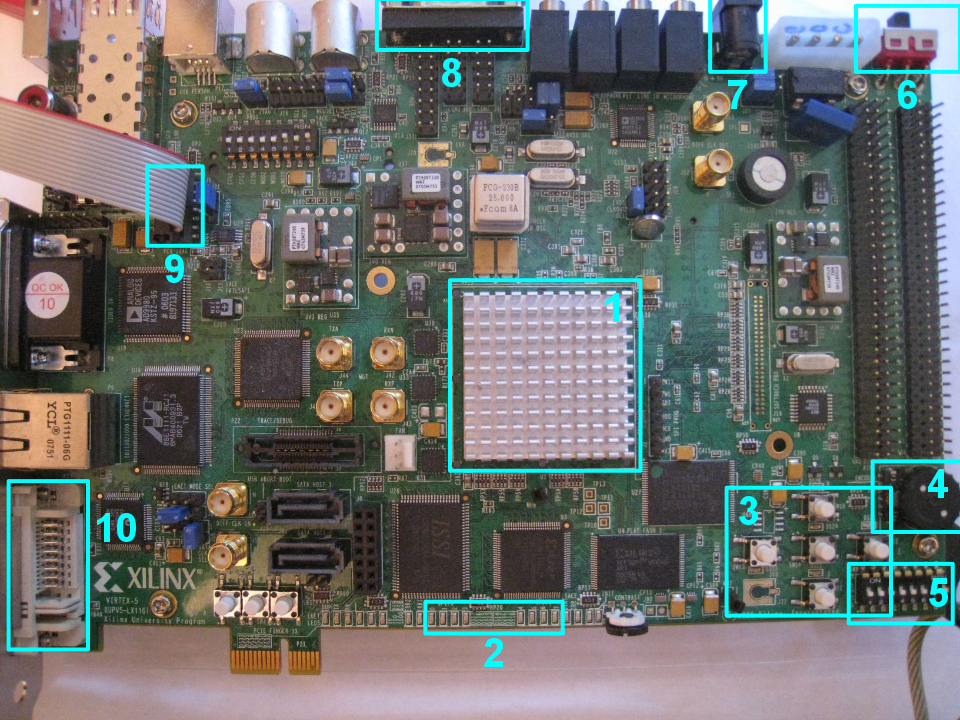
\includegraphics[width=\textwidth]{images/dev_board.png}
\begin{enumerate}
	\item Virtex-5 FPGA (covered by heat sink). It is connected to the peripheral ICs and I/O connectors via PCB traces.
	\item GPIO LEDs, numbered 0-7
	\item North, East, South, West, Center user push buttons, each with a corresponding LED
	\item Rotary encoder (a wheel we can rotate clockwise or counterclockwise and push horizontally)
	\item GPIO DIP (dual-inline package) switches, numbered 1-8 (but referred to 0-7 in code)
	\item Board power switch (toggle for a full board reset, after which you will have to reprogram the FPGA)
	\item Power connector; the power cable on many of these board is sensitive to movement and can come loose easily. Make sure you seat the power cable properly.
	\item Serial port
	\item JTAG header (used to program the FPGA, the Xilinx programmer is connected to this header)
	\item DVI-I connector (for video output)
\end{enumerate}

You will also notice a device sitting to the left of the development board that looks like this:\\

\begin{center}
	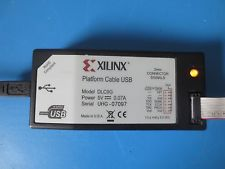
\includegraphics{images/xilinx_platform_cable.jpg}
\end{center}

This is a Xilinx FPGA programmer that connects to your workstation (desktop computer) over USB to receive a compiled bitstream file which it then sends to the development board and the FPGA over the JTAG interface. Before you run \verb|make impact| to send your design to the FPGA, make sure that the LED on the programmer is glowing green. If it is glowing yellow or not glowing at all, make sure that the wired connections are solid and that the development board is powered and on.

\section{The FPGA - Xilinx Virtex-5 LX110T}
To help you become familiar with the FPGA that you will be working with through the semester, please read Chapter 5: Configurable Logic Blocks (page 171) of the \href{http://inst.eecs.berkeley.edu/~cs150/fa11/resources/ug190.pdf}{Virtex-5 User Guide} and answer the following questions (you should be able to discuss your answers for checkoff):

\subsection{Checkoff Questions}
\begin{enumerate}
	\item How many SLICEs are in a single CLB?
	\item How many inputs do each of the LUTs on a Virtex-5 LX110T FPGA have?
	\item How many LUTs does the LX110T have?
	\item How do you implement logic functions of 7 inputs in a single SLICEL? How about 8? Draw a high-level circuit diagram to show how the implementation would look. Be specific about the elements (LUTs, muxes) that are used.
	\item What is the difference between a SLICEL and a SLICEM?
\end{enumerate}

\section{Overview of the FPGA Build Toolchain}
Before we begin the lab, we should familiarize ourselves with the CAD (computer aided design) tools that translate HDL into a working circuit on the FPGA. These tools will pass your design through several stages, each one bringing it closer to a concrete implementation.\\

Looking at the directory structure of the \verb|lab1| folder, you can see two main folders, \verb|src| and \verb|cfg|. You will also find a \verb|Makefile|. When executing parts of the toolchain, you will want to run \verb|make| in the \verb|lab1| folder. The \verb|Makefile| delegates to another \verb|Makefile| that resides in the \verb|cfg| folder. In the \verb|cfg| folder you will also find other files that are used by tools during the build process. We will discuss every step of the toolchain.\\

\subsection{Synthesis}
The synthesis tool (in this case of this class, Xilinx Synthesis Tool(xst)) is the first program that processes your design. Among other tasks, it is responsible for the process of transforming the primitive gates and flip-flops that you wrote in Verilog into LUTs and other primitive FPGA elements.\\

For example, if you described a circuit composed of many gates, but ultimately of 6 inputs and 1 output, xst will map your circuit down to a single 6-LUT. Likewise, if you described a flip-flop it will be mapped to a specific type of flip-flop which actually exists on the FPGA.\\

The following figure shows the flow of files through XST. \\

\begin{center}
	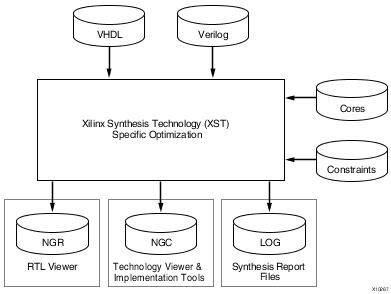
\includegraphics{images/xst_design_flow.png}
\end{center}

XST takes in Verilog and/or VHDL files to be parsed and synthesized.

XST also takes in 'Cores' which are pre-built and synthesized digital circuit blocks that provide some commonly needed functionality; they are usually provided by Xilinx to enable rapid FPGA development. They include things like pipelined dividers and multipliers, floating point units, and system buses.

XST also takes in 'Constraints' which are given in the form of a XCF file. In this lab, we don't use any constraints or cores that are passed into XST.

The outputs of XST include a LOG file, which is a text file that you can examine to make sure the synthesis succeeded, or if it failed or emitted warnings, you can see what those issues are.

Another output of XST is a NGR file which can be viewed with Xilinx ISE (as we will see soon); this file gives a high-level schematic view of how your Verilog modules are set to be implemented on the FPGA.

The final product of synthesis is a netlist file (NGC); it is a text file that contains a list of all the instances of primitive components in the translated circuit and a description of how they are connected.

\subsection{Translation and Mapping}
The tools that perform translation and mapping are NGDBuild and Map respectively. These tools take the output of the synthesis tool (a generic netlist) and translates each component to an equivalent on the specific Xilinx vc5vlx110t FPGAs we have in the lab. 

The translation tool merges all the input netlists and design constraint information and outputs a Xilinx Native Generic Database (NGD) file. NGDBuild takes the UCF (User Constraints File) and the NGC (from XST) files as inputs.

The mapping tool maps the logic defined by an NGD file into FPGA elements such as CLBs (configurable logic blocks) and IOBs (input/output blocks). The Map tool takes in the NGD file produced by the translation tool and produces a Xilinx Native Circuit Description (NCD) file.

\subsubsection{User Constraints File (UCF)}
We will take a small detour here to cover what a UCF is and how to add top-level signal connections to it.

\subsection{Place and Route}

\section{A Structural and Behavioral Adder Design + Using fpga\_editor and the FPGA schematic}

\section{Designing a Tone Generator}

\subsection{Piezoelectronic Buzzers}

\subsection{Finding the Piezo in the Schematic}

\subsection{Adding the Piezo signal to the UCF File}

\subsection{Generating a square wave}

\subsection{Switching the Wave On and Off}

\section{}

\end{document}
